\documentclass{article}
\usepackage{import}
\import{../../../lib/latex/}{wgmlgz}


\begin{document}

\itmo[
  variant=19489,
  labn=4,
  discipline=Основы профессиональной деятельности,
  group=P3115,
  student=Владимир Мацюк,
  teacher=Абузов Ярослав Александрович,
  logo=../../../lib/img/itmo.png
]

\section{Текст задания}
По выданному преподавателем варианту восстановить текст заданного варианта программы, определить предназначение и составить описание программы, определить область представления и область допустимых значений исходных данных и результата, выполнить трассировку программы.
\begin{center}
  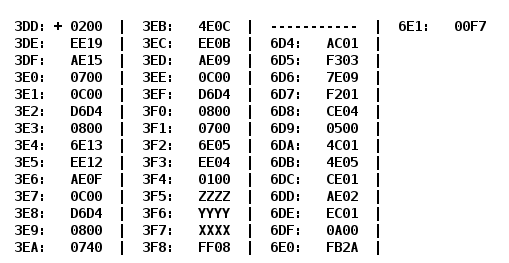
\includegraphics[scale=0.8]{task.png}
\end{center}
\begin{tabular}{|c|r|l|l|} \hline
  Адрес & Код команды & Мнемоника       & Комментарии \nl
  3DD   & +0200       & CLA             & Очистка аккумулятора \nl
  3DE   & EE19        & ST IP+19  (r)   & Сохранение (Прямая относительная адресация) \nl
  3DF   & AE15        & LD IP+15  (z)   & Загрузка (Прямая относительная адресация) \nl
  3E0   & 0700        & INC             & Инкремент \nl
  3E1   & 0C00        & PUSH            & Запись в стэк \nl
  3E2   & D6D4        & CALL 0x6D4      & Вызов подпрограммы (Прямая абсолютная адресация) \nl
  3E3   & 0800        & POP             & Чтение из стэка \nl

  3E4   & 6E13        & SUB IP+13 (r)   & Вычитание (Прямая относительная адресация) \nl
  3E5   & EE12        & ST IP+12 (r)    & Сохранение (Прямая относительная адресация) \nl
  3E6   & AE0F        & LD IP+F  (y)    & Загрузка (Прямая относительная адресация) \nl
  3E7   & 0C00        & PUSH            & Запись в стэк \nl
  3E8   & D6D4        & CALL 0x6D4      & Вызов подпрограммы (Прямая абсолютная адресация) \nl
  3E9   & 0800        & POP             & Чтение из стэка \nl

  3EA   & 0740        & DEC             & Декремент \nl
  3EB   & 4E0C        & ADD IP+C (r)    & Сложение (Прямая относительная адресация) \nl
  3EC   & EE0B        & ST IP+B  (r)    & Сохранение (Прямая относительная адресация) \nl
  3ED   & AE09        & LD IP+9 (x)     & Загрузка (Прямая относительная адресация) \nl
  3EE   & 0C00        & PUSH            & Запись в стэк \nl
  3EF   & D6D4        & CALL 0x6D4      & Вызов подпрограммы (Прямая абсолютная адресация) \nl
  3F0   & 0800        & POP             & Чтение из стэка \nl

  3F1   & 0700        & INC             & Инкремент \nl
  3F2   & 6E05        & SUB IP+5 (r)    & Вычитание (Прямая относительная адресация) \nl
  3F3   & EE04        & ST IP+4  (r)    & Сохранение (Прямая относительная адресация) \nl
  3F4   & 0100        & HLT             & Остановка \nl

  3F5   & ZZZZ        & константа       & z \nl
  3F6   & YYYY        & константа       & y \nl
  3F7   & XXXX        & константа       & x \nl
  3F8   & FF08        & переменная      & r \nl
  6D4   & AC01        & LD (SP+1)       & Загрузка (Косвенная относительная со смещением) \nl
  605   & F303        & BPL IP+3 (a)    & Переход, если плюс \nl
  6D6   & 7E09        & CMP IP+9 (A)    & Сравнение (Прямая относительная адресация) \nl
  6D7   & F201        & BMI IP+1 (a)    & Переход, если минус \nl
  6D8   & CE04        & BR IP+4 (b)     & Безусловный переход (эквивалент JUMP c прямой относительной адресацией) \nl
  6D9   & 0500        & a: ASL          & Арифметический сдвиг влево \nl
  6DA   & 4C01        & ADD (SP+1)      & Сложение (Косвенная относительная со смещением) \nl
  6DB   & 4E05        & ADD IP+5  (B)   & Сложение (Прямая относительная адресация) \nl
  6DC   & CE01        & BR IP+1 (c)     & Безусловный переход (эквивалент JUMP c прямой относительной адресацией) \nl
  6DD   & AE02        & b: LD IP+2  (A) & Загрузка (Прямая относительная адресация) \nl
  6DE   & EC01        & c: ST (SP+1)    & Сохранение (Косвенная относительная со смещением) \nl
  6DF   & 0A00        & RET             & Возврат из подпрограммы \nl
  6E0   & FB2A        & константа       & A\nl
  6E1   & 00F7        & константа       & B\nl
\end{tabular}

\section{Описание программы}

Программа находит количесво отрицательных чисел и сохраняет результат в ячейке 4D3.
Псевдокод:


% asm


% \begin{lstlisting}

% ac = 0
% t = ac
% ac = z
% ++ac
% ac = f(ac)

% ac -= t
% t = ac
% ac = y
% ac = f(ac)

% --ac
% ac += t
% t = ac
% ac = x
% ac = f(ac)

% ++ac
% ac -= t

% \end{lstlisting}




% \begin{lstlisting}

%   ac = arg
%   if ac > 0: jpm a
%   cmp A
%   if ac < 0: jmp a

%   jmp b

%   a: ac <<= 1
%   ac += arg
%   ac += B
%   jmp c

%   b: ac = a

%   c: arg = ac
%   ret 


% \end{lstlisting}


% c


% \begin{lstlisting}

% ac = 0
% t = ac
% ac = z
% ++ac
% ac = f(ac)

% ac -= t
% t = ac
% ac = y
% ac = f(ac)

% --ac
% ac += t
% t = ac
% ac = x
% ac = f(ac)

% ++ac
% ac -= t
% t = ac


% \end{lstlisting}


% \begin{lstlisting}
% f(x)
%   ac = x
%   if ac >= 0  ac < A
%     ac <<= 1
%     ac += x
%     ac += B
%   else
%     ac = a

%   return ac 
% \end{lstlisting}

% js


\begin{lstlisting}
t = 0
t = f(z + 1) - t
t = f(y) - 1 + t
t = f(x) + 1 - t
\end{lstlisting}
\begin{lstlisting}
f = (x) => (x >= 0 | x < A) ? 3x + B : A
\end{lstlisting}

$$
  f(x) = \begin{cases}
    3x + B,\  x \ge 0\ |\ x < A \\
    A
  \end{cases}
$$
$$   A = -1238,\ B = 247$$
$$    R = f(x) - f(y) - f(z + 1) + 2 $$
\begin{center}
  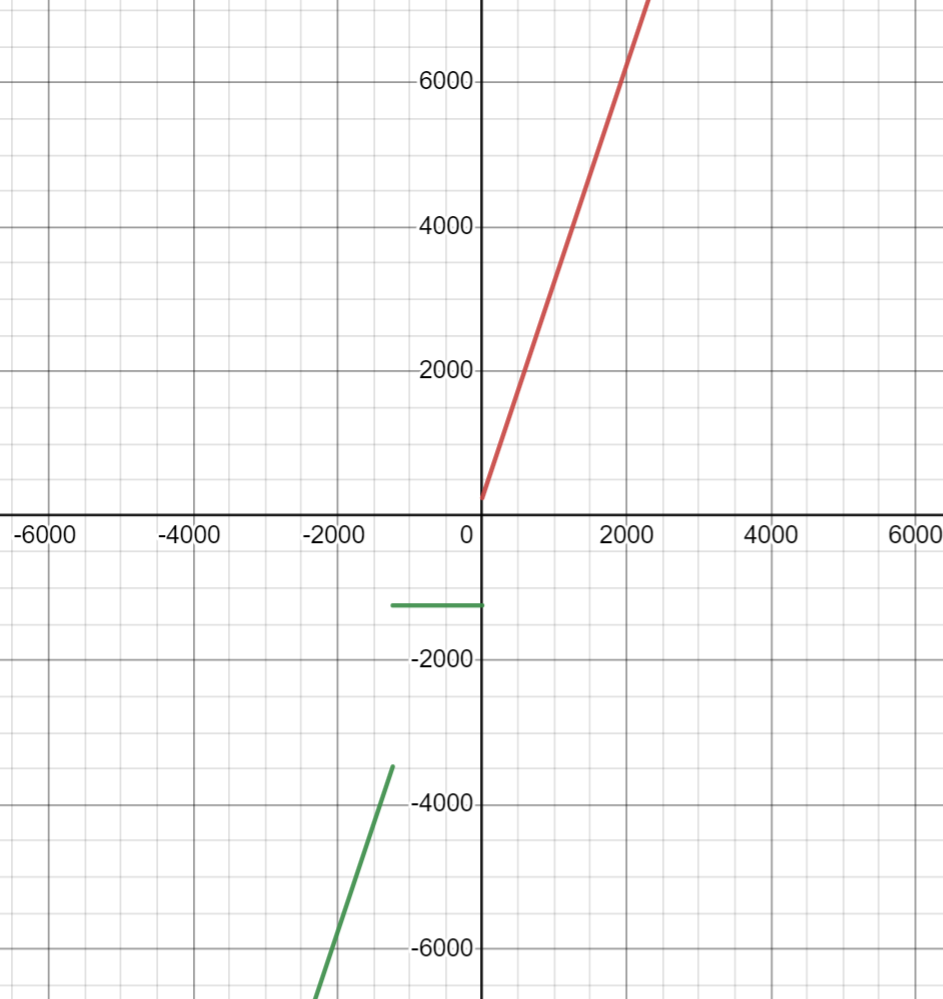
\includegraphics[scale=0.8]{graph.png}
\end{center}
\section{Область представления}
\begin{itemize}
  \item x, y, z, r, a, b - целые знаковые шестнадцатеричные числа
\end{itemize}

\section{Расположение данных в памяти}

\begin{itemize}
  \item Основная программа:
        \begin{itemize}
          \item 3DD-3F4 – команды;
          \item 3F5, 3F6, 3F7 – исходные данные;
          \item 3F8 – итоговый результат.
        \end{itemize}
  \item Подпрограмма:
        \begin{itemize}
          \item 6D4-6DF – команды;
          \item 6E0, 6E1 – переменные.
        \end{itemize}
\end{itemize}

\section{Адреса первой и последней выполняемой команды}

\begin{itemize}
  \item Основная программа:
        \begin{itemize}
          \item Адрес первой команды: 3DD
          \item Адрес последней команды: 3F4
        \end{itemize}
  \item Подпрограмма:
        \begin{itemize}
          \item Адрес первой команды: 6D4
          \item Адрес последней команды: 6E1
        \end{itemize}
\end{itemize}


\section{Область представления}

Область допустимых значений
A = -1238
B = 247

Для того чтобы определить одз, проанализируем данную функцию. При значении аргумента функции в промежутке $(-1238; 0]$, функция вернет значение выражения A. При использовании любого значения из заданного промежутка в функции не возникнет переполнения. При оставшихся значениях аргумента функция вернет выражение 3*x+B, что означает, что функция не переполняется на промежутке $[-10840, -11005]$, а в других случаях будет переполнение.
$$ f_{min}=f\left(-10840\right)=-32273 $$
$$ f_{max}\ =\ f(10840)\ =\ 32767 $$
Однако данные числа максимальные, чтобы не было переполнения.
Так как основная программа вычисляет следующее выражение:

$$ r = f(x) - f(y) - f(z + 1) + 2 $$

То минимально мы можем получить $-32766 -32766 - 32766 = -98298 < -2^{15}$

А максимально: $32766 + 32766 + 32766 = 98298 > 2^{15} – 1$
В обоих случаях переполнение возможно.

В функцию как аргументы мы передаем значения $Z+1, Y, X$.

Значит, одз:
$$ \begin{cases}
    \frac{-2^{15}}{3} \le X \le \frac{2^{15} - 1}{3} \\
    \frac{-2^{15}}{3} \le Y \le \frac{2^{15} - 1}{3} \\
    \frac{-2^{15} - 1}{3} \le Z \le \frac{2^{15}}{3} \\
  \end{cases}\,.
$$

\section{Таблица трассировки}

\begin{tabular}{|c|c|c|c|c|c|c|c|c|c|c|c|c|c|c|} \hline
  Адр & Код  & IP  & CR   & AR  & DR   & SP  & BR   & AC   & PS  & NZVC & Адр & Код \nl
  3DD & 0200 & 3DD & 0000 & 000 & 0000 & 000 & 0000 & 0000 & 004 & 0100 & \nl
  3DD & 0200 & 3DE & 0200 & 3DD & 0200 & 000 & 03DD & 0000 & 004 & 0100 & \nl
  3DE & EE19 & 3DF & EE19 & 3F8 & 0000 & 000 & 0019 & 0000 & 004 & 0100 & 3F8 & 0000 \nl
  3DF & AE15 & 3E0 & AE15 & 3F5 & 0028 & 000 & 0015 & 0028 & 000 & 0000 & \nl
  3E0 & 0700 & 3E1 & 0700 & 3E0 & 0700 & 000 & 03E0 & 0029 & 000 & 0000 & \nl
  3E1 & 0C00 & 3E2 & 0C00 & 7FF & 0029 & 7FF & 03E1 & 0029 & 000 & 0000 & 7FF & 0029 \nl
  3E2 & D6D4 & 6D4 & D6D4 & 7FE & 03E3 & 7FE & D6D4 & 0029 & 000 & 0000 & 7FE & 03E3 \nl
  6D4 & AC01 & 6D5 & AC01 & 7FF & 0029 & 7FE & 0001 & 0029 & 000 & 0000 & \nl
  6D5 & F303 & 6D9 & F303 & 6D5 & F303 & 7FE & 0003 & 0029 & 000 & 0000 & \nl
  6D9 & 0500 & 6DA & 0500 & 6D9 & 0029 & 7FE & 06D9 & 0052 & 000 & 0000 & \nl
  6DA & 4C01 & 6DB & 4C01 & 7FF & 0029 & 7FE & 0001 & 007B & 000 & 0000 & \nl
  6DB & 4E05 & 6DC & 4E05 & 6E1 & 00F7 & 7FE & 0005 & 0172 & 000 & 0000 & \nl
  6DC & CE01 & 6DE & CE01 & 6DC & 06DE & 7FE & 0001 & 0172 & 000 & 0000 & \nl
  6DE & EC01 & 6DF & EC01 & 7FF & 0172 & 7FE & 0001 & 0172 & 000 & 0000 & 7FF & 0172 \nl
  6DF & 0A00 & 3E3 & 0A00 & 7FE & 03E3 & 7FF & 06DF & 0172 & 000 & 0000 & \nl
  3E3 & 0800 & 3E4 & 0800 & 7FF & 0172 & 000 & 03E3 & 0172 & 000 & 0000 & \nl
  3E4 & 6E13 & 3E5 & 6E13 & 3F8 & 0000 & 000 & 0013 & 0172 & 001 & 0001 & \nl
  3E5 & EE12 & 3E6 & EE12 & 3F8 & 0172 & 000 & 0012 & 0172 & 001 & 0001 & 3F8 & 0172 \nl
  3E6 & AE0F & 3E7 & AE0F & 3F6 & 0028 & 000 & 000F & 0028 & 001 & 0001 & \nl
  3E7 & 0C00 & 3E8 & 0C00 & 7FF & 0028 & 7FF & 03E7 & 0028 & 001 & 0001 & 7FF & 0028 \nl
  3E8 & D6D4 & 6D4 & D6D4 & 7FE & 03E9 & 7FE & D6D4 & 0028 & 001 & 0001 & 7FE & 03E9 \nl
  6D4 & AC01 & 6D5 & AC01 & 7FF & 0028 & 7FE & 0001 & 0028 & 001 & 0001 & \nl
  6D5 & F303 & 6D9 & F303 & 6D5 & F303 & 7FE & 0003 & 0028 & 001 & 0001 & \nl
  6D9 & 0500 & 6DA & 0500 & 6D9 & 0028 & 7FE & 06D9 & 0050 & 000 & 0000 & \nl
  6DA & 4C01 & 6DB & 4C01 & 7FF & 0028 & 7FE & 0001 & 0078 & 000 & 0000 & \nl
  6DB & 4E05 & 6DC & 4E05 & 6E1 & 00F7 & 7FE & 0005 & 016F & 000 & 0000 & \nl
  6DC & CE01 & 6DE & CE01 & 6DC & 06DE & 7FE & 0001 & 016F & 000 & 0000 & \nl
  6DE & EC01 & 6DF & EC01 & 7FF & 016F & 7FE & 0001 & 016F & 000 & 0000 & 7FF & 016F \nl
  6DF & 0A00 & 3E9 & 0A00 & 7FE & 03E9 & 7FF & 06DF & 016F & 000 & 0000 & \nl
  3E9 & 0800 & 3EA & 0800 & 7FF & 016F & 000 & 03E9 & 016F & 000 & 0000 & \nl
  3EA & 0740 & 3EB & 0740 & 3EA & 0740 & 000 & 03EA & 016E & 001 & 0001 & \nl
  3EB & 4E0C & 3EC & 4E0C & 3F8 & 0172 & 000 & 000C & 02E0 & 000 & 0000 & \nl
  3EC & EE0B & 3ED & EE0B & 3F8 & 02E0 & 000 & 000B & 02E0 & 000 & 0000 & 3F8 & 02E0 \nl
  3ED & AE09 & 3EE & AE09 & 3F7 & 0028 & 000 & 0009 & 0028 & 000 & 0000 & \nl
  3EE & 0C00 & 3EF & 0C00 & 7FF & 0028 & 7FF & 03EE & 0028 & 000 & 0000 & 7FF & 0028 \nl
  3EF & D6D4 & 6D4 & D6D4 & 7FE & 03F0 & 7FE & D6D4 & 0028 & 000 & 0000 & 7FE & 03F0 \nl
  6D4 & AC01 & 6D5 & AC01 & 7FF & 0028 & 7FE & 0001 & 0028 & 000 & 0000 & \nl
  6D5 & F303 & 6D9 & F303 & 6D5 & F303 & 7FE & 0003 & 0028 & 000 & 0000 & \nl
  6D9 & 0500 & 6DA & 0500 & 6D9 & 0028 & 7FE & 06D9 & 0050 & 000 & 0000 & \nl
  6DA & 4C01 & 6DB & 4C01 & 7FF & 0028 & 7FE & 0001 & 0078 & 000 & 0000 & \nl
  6DB & 4E05 & 6DC & 4E05 & 6E1 & 00F7 & 7FE & 0005 & 016F & 000 & 0000 & \nl
  6DC & CE01 & 6DE & CE01 & 6DC & 06DE & 7FE & 0001 & 016F & 000 & 0000 & \nl
  6DE & EC01 & 6DF & EC01 & 7FF & 016F & 7FE & 0001 & 016F & 000 & 0000 & 7FF & 016F \nl
  6DF & 0A00 & 3F0 & 0A00 & 7FE & 03F0 & 7FF & 06DF & 016F & 000 & 0000 & \nl
  3F0 & 0800 & 3F1 & 0800 & 7FF & 016F & 000 & 03F0 & 016F & 000 & 0000 & \nl
  3F1 & 0700 & 3F2 & 0700 & 3F1 & 0700 & 000 & 03F1 & 0170 & 000 & 0000 & \nl
  3F2 & 6E05 & 3F3 & 6E05 & 3F8 & 02E0 & 000 & 0005 & FE90 & 008 & 1000 & \nl
  3F3 & EE04 & 3F4 & EE04 & 3F8 & FE90 & 000 & 0004 & FE90 & 008 & 1000 & 3F8 & FE90 \nl
  3F4 & 0100 & 3F5 & 0100 & 3F4 & 0100 & 000 & 03F4 & FE90 & 008 & 1000 & \nl
\end{tabular}

\section{Вывод}

Во время выполнения лабораторной работы я научился вызывать и исследовать подпрограммы, работать
со стеком, изучил цикл выполнения таких команд как CALL и RET.

\end{document}
